\documentclass[unicode,11pt,a4paper,oneside,numbers=endperiod,openany]{scrartcl}
\usepackage[utf8]{inputenc}  % Allows UTF-8 input (for special characters, etc.)
\usepackage{amsmath}         % Provides advanced math features
\usepackage{amssymb}         % For additional math symbols
\usepackage{graphicx}        % Allows including images
\usepackage{array}           % For tables
\usepackage{geometry}        % To adjust page margins
\usepackage{hyperref}        % For links and references
\usepackage{fancyhdr}        % For customized headers and footers
\usepackage{multicol}        % For multiple columns
\usepackage{verbatim}        % For verbatim text (like the gene sequence)
\usepackage{longtable}       % For long tables that span multiple pages
\usepackage{xcolor}          % For colored text (if needed)
\usepackage{listings}
\usepackage{dnaseq}         % For DNA sequences
\usepackage{amsmath}
\usepackage{float}  % To prevent floating of figures
\usepackage{lmodern}
\usepackage{listings}
\usepackage{pdfpages}
\usepackage{seqsplit}
\usepackage{subcaption} % For side-by-side captions
\usepackage{placeins}
\usepackage{amsmath}
\usepackage{ifthen}
\usepackage[utf8]{inputenc}
\usepackage{graphics}
\usepackage{graphicx}
\usepackage{hyperref}

\pagestyle{plain}
\voffset -5mm
\oddsidemargin  0mm
\evensidemargin -11mm
\marginparwidth 2cm
\marginparsep 0pt
\topmargin 0mm
\headheight 0pt
\headsep 0pt
\topskip 0pt        
\textheight 255mm
\textwidth 165mm

\newcommand{\duedate} {}
\newcommand{\setduedate}[1]{%
\renewcommand\duedate {See iCorsi for due date}}
\newcommand\isassignment {false}
\newcommand{\setassignment}{\renewcommand\isassignment {true}}
\newcommand{\ifassignment}[1]{\ifthenelse{\boolean{\isassignment}}{#1}{}}
\newcommand{\ifnotassignment}[1]{\ifthenelse{\boolean{\isassignment}}{}{#1}}

\newcommand{\assignmentpolicy}{
\begin{table}[h]
\begin{center}
\scalebox{0.8} {%
\begin{tabular}{|p{0.02cm}p{16cm}|}
\hline
&\\
\multicolumn{2}{|c|}{\Large\textbf{HPC Lab ---  Submission Instructions}}\\
\multicolumn{2}{|c|}{\large\textbf{(Please, notice that following instructions are mandatory: }}\\
\multicolumn{2}{|c|}{\large\textbf{submissions that don't comply with, won't be considered)}}\\
&\\
\textbullet & Assignments must be submitted to \href{https://www.icorsi.ch}{iCorsi} (i.e. in electronic format).\\
\textbullet & Provide both executable package and sources (e.g. C/C++ files, Matlab). 
If you are using libraries, please add them in the file. Sources must be organized in directories called:\\
\multicolumn{2}{|c|}{\textit{Project\_number\_lastname\_firstname}}\\
& and  the  file must be called:\\
\multicolumn{2}{|c|}{\textit{project\_number\_lastname\_firstname.zip}}\\
\multicolumn{2}{|c|}{\textit{project\_number\_lastname\_firstname.pdf}}\\
\textbullet &  The TAs will grade your project by reviewing your project write-up, and looking at the implementation 
                 you attempted, and benchmarking your code's performance.\\

\textbullet & You are allowed to discuss all questions with anyone you like; however: (i) your submission must list anyone you discussed problems with and (ii) you must write up your submission independently.\\
\hline
\end{tabular}
}
\end{center}
\end{table}
}
\newcommand{\punkte}[1]{\hspace{1ex}\emph{\mdseries\hfill(#1~\ifcase#1{Points}\or{Points}\else{Points}\fi)}}


\newcommand\serieheader[6]{
\thispagestyle{empty}%
\begin{flushleft}

\includegraphics[width=0.4\textwidth]{usi_inf.png}
\end{flushleft}
  \noindent%
  {\large\ignorespaces{\textbf{#1}}\hspace{\fill}\ignorespaces{ \textbf{#2}}}\\ \\%
  {\large\ignorespaces #3 \hspace{\fill}\ignorespaces #4}\\
  \noindent%
  \bigskip
  \hrule\par\bigskip\noindent%
  \bigskip {\ignorespaces {\Large{\textbf{#5}}}
  \hspace{\fill}\ignorespaces \large \ifthenelse{\boolean{\isassignment}}{\duedate}{#6}}
  \hrule\par\bigskip\noindent%  \linebreak
 }

\makeatletter
\def\enumerateMod{\ifnum \@enumdepth >3 \@toodeep\else
      \advance\@enumdepth \@ne
      \edef\@enumctr{enum\romannumeral\the\@enumdepth}\list
      {\csname label\@enumctr\endcsname}{\usecounter
        {\@enumctr}%%%? the following differs from "enumerate"
	\topsep0pt%
	\partopsep0pt%
	\itemsep0pt%
	\def\makelabel##1{\hss\llap{##1}}}\fi}
\let\endenumerateMod =\endlist
\makeatother




\usepackage{textcomp}





\begin{document}


\setassignment

\serieheader{High-Performance Computing Lab}{Institute of Computing}{Student: JONATAN BELLA}{Discussed with: NONE}{Solution for Project 5}{}
\newline

\assignmentpolicy
This project will introduce you a parallel space solution of a nonlinear PDE using MPI.

% -------------------------------------------------------------------------- %
% -------------------------------------------------------------------------- %
% ---------------------- Exercise 1 -----------------------------------------%
% -------------------------------------------------------------------------- %
% -------------------------------------------------------------------------- %

\section{Task 1 - Initialize and finalize MPI [5 Points]}

As on previous assignments, I first initialize the MPI environment with \texttt{MPI\_Init()}.
I define the respective rank and size variables of the process and pass them to
the communication functions \texttt{MPI\_Comm\_rank()} and \texttt{MPI\_Comm\_size()}.

Now, to make one rank to print the welcome message, I check if the rank is 0 and print all related messages
(metadata, summarizing table and welcome message - with the process added to the print). Finally, i added
the finalization of the MPI environment with \texttt{MPI\_Finalize()} before the return as expected.

To run the respective files, I change the compiler to "mpicxx" in the Makefile and I run the 
following command for testing: "mpirun -np 4 ./main 128 100 0.005".

\section{Task 2 - Create a Cartesian topology [10 Points]}

As in the previous task, I import the MPI library and define the respective rank and size variables.
Then, I make use of the \texttt{MPI\_Dims\_create()} function to create a 2D, non-periodic given input variables, 
Cartesian topology such that it automatically determine the optimal process grid size. As an example, 
4 processes with 128x128 grid size should be organized in a 64x64 grid. 

Then, I proceed to establish the communication topology using \texttt{MPI\_Cart\_create()}, where I pass the 
dimensions, the periodicity and the communicator. To map the processes to the respective grid positions, 
I use \texttt{MPI\_Cart\_coords()} to get the coordinates of the respective process such that
each process knows its position in the grid. As in this case, Rank 0 would obtain position (1,1) - bottom left
whereas Rank 1 would obtain (2,1) - bottom right and so on.

Finally, I set the neighbors for all directions using \texttt{MPI\_Cart\_shift()}.
Where one manage the South-North neighbors and the other one the West-East neighbors.
Finally, I free the Cartesian communicator using \texttt{MPI\_Comm\_free()}.

As a final comment on the results, the code shows the expected positioning and grid size:

\begin{verbatim}
version   :: C++ MPI
processes :: 4
mesh      :: 128 * 128 dx = 0.00787402
time      :: 100 time steps from 0 .. 0.005
iteration :: CG 300, Newton 50, tolerance 1e-06
================================================================================
rank 1 / 4 : (2, 1) neigh N:S 3:-2 neigh E:W -2:0 local dims 64 x 64
rank 2 / 4 : (1, 2) neigh N:S -2:0 neigh E:W 3:-2 local dims 64 x 64
rank 3 / 4 : (2, 2) neigh N:S -2:1 neigh E:W -2:2 local dims 64 x 64
\end{verbatim}

Meaning that perfect balance is achieved since each process handles the 64x64 points, which
theoretically should evenly distribute the computational load. Since $MPI\_Dims\_create$ works
with any process count and handles arbitrary grid sizes then the code is scalable. 
Notice that -2 in the output indicates the boundaries. 


\section{Task 3 - Change linear algebra functions [5 Points]}

There are only two functions that needs the accumulated operations to be performed. 
One is the dot product and the other one is the norm. In the first case, we need to 
accumulate all the partial inner products. For this I use the \texttt{MPI\_Allreduce()} function
which performs a global reduction of the partial results. 

\begin{verbatim}
  double global_result = 0;
  MPI_Allreduce(&result, &global_result, 1, MPI_DOUBLE, MPI_SUM, MPI_COMM_WORLD);
  return global_result;
\end{verbatim}

In the second case, and similar to the dot product, I perform a global sum
of the partial results of the norms and return the square root of it, as any euclidean norm calculation.

\begin{verbatim}
double global_result = 0;
MPI_Allreduce(&result, &global_result, 1, MPI_DOUBLE, MPI_SUM, MPI_COMM_WORLD);
return sqrt(global_result);
\end{verbatim}

\section{Task 4 - Exchange ghost cells [45 Points] }

For this implementation, and as a first general overview, we need to check for neighbors on each direction and post 
a non-blocking receive to get the data from that neighbor. Then, we copy our boundary data into a send buffer that we use 
in a non-blocking send to send our data to the neighbour. Finally, we wait for all communications to complete using 
\texttt{MPI\_Waitall()}. To have a picture in mind of what we need to do, imagining we have 4 processes and process 0 have the grid of top 
left whereas process two the bottom-left, then as an example, process 0 needs to send its bottom row to process 2 to complete its calculations
and receive the top row from process 2 to complete its calculations. Therefore, $domain.neighbour\_south >= 0$ would return true for process 0 in this example.
Then, it will proceed to receive the data from the bottom neighbor, then copy the information of the bottom row of this process to finally
be send to process 2.
In consequence, For the north and south neighbors we need to use the nx doubles (rows) whereas for the east and west ones,
we need the ny doubles (columns). Therefore, the inputs for the $MPI\_Irecv$ and $MPI\_Isend$ are the following:
the destination buffer where the data will be stored, the number of elements to be received/sent, the data type, the rank of the source process,
the tag of the message, the communicator and the request handle indexed by the variable $num\_requests$ which is incremented by 1 for each request.
Notice that we have 8 requests in total, 2 for each direction (send and receive - N, S, E, W).

\begin{verbatim}
  // North neighbor exchange
  if (domain.neighbour_north >= 0) {
      // we receive from north -> non blocking receive first 
      MPI_Irecv(&bndN[0], nx, MPI_DOUBLE, domain.neighbour_north, 
                domain.neighbour_north, MPI_COMM_WORLD, &requests[num_requests++]);
      
      // copy into north buffer
      for (int i = 0; i < nx; i++) 
          buffN[i] = s_new(i, ny-1);
      
      // send to north -> and post the non blocking send
      MPI_Isend(&buffN[0], nx, MPI_DOUBLE, domain.neighbour_north,
                domain.rank, MPI_COMM_WORLD, &requests[num_requests++]);
  }

  // South neighbor exchange
  if (domain.neighbour_south >= 0) {
      // we receive from south
      MPI_Irecv(&bndS[0], nx, MPI_DOUBLE, domain.neighbour_south,
                domain.neighbour_south, MPI_COMM_WORLD, &requests[num_requests++]);
      
      // copy into south buffer
      for (int i = 0; i < nx; i++)
          buffS[i] = s_new(i, 0);
      
      // send to south
      MPI_Isend(&buffS[0], nx, MPI_DOUBLE, domain.neighbour_south,
                domain.rank, MPI_COMM_WORLD, &requests[num_requests++]);
  }

  // East neighbor exchange
  if (domain.neighbour_east >= 0) {
      // we receive from east
      MPI_Irecv(&bndE[0], ny, MPI_DOUBLE, domain.neighbour_east,
                domain.neighbour_east, MPI_COMM_WORLD, &requests[num_requests++]);
      
      // copy into east buffer
      for (int j = 0; j < ny; j++)
          buffE[j] = s_new(nx-1, j);
      
      // send to east
      MPI_Isend(&buffE[0], ny, MPI_DOUBLE, domain.neighbour_east,
                domain.rank, MPI_COMM_WORLD, &requests[num_requests++]);
  }

  // West neighbor exchange
  if (domain.neighbour_west >= 0) {
      // we receive from west
      MPI_Irecv(&bndW[0], ny, MPI_DOUBLE, domain.neighbour_west,
                domain.neighbour_west, MPI_COMM_WORLD, &requests[num_requests++]);
      
      // copy into west buffer
      for (int j = 0; j < ny; j++)
          buffW[j] = s_new(0, j);
      
      // send to west
      MPI_Isend(&buffW[0], ny, MPI_DOUBLE, domain.neighbour_west,
                domain.rank, MPI_COMM_WORLD, &requests[num_requests++]);
  }
\end{verbatim}

The request handles are essential for the $MPI\_Waitall()$ function to know which requests to wait for. 
Which is call after the inner points computations that do not need to use Ghost cells since this ghost cells
will be necessary for the boundaries. This allows us, while the messages are being sent and receive, we can compute the
inner points in parallel, reducing / overlapping the communication latency and using the time as most efficient as possible. 


\section{Task 5 - Implement parallel I/O [10 Points]}
To implement this task, i follow closely the provided example. 
First, i create the binary file name and open the file with the appropriate flags such
that all processes open the file. Then, i create a subarray datatype for this process portion of the grid.

\begin{verbatim}
MPI_File filehandle;
MPI_File_open(MPI_COMM_WORLD, fname_bin.c_str(), 
              MPI_MODE_CREATE | MPI_MODE_WRONLY,
              MPI_INFO_NULL, &filehandle);
\end{verbatim}

This subarray describes each process portion and handles the appropriate positioning in the global array as row-major
ordering. Therefore, it is where we define how the local data maps to the global file.

\begin{verbatim}
int sizes[2]    = {options.nx, options.nx};  // global grid size
int subsizes[2] = {domain.nx, domain.ny};    // local grid size
int starts[2]   = {domain.startx-1, domain.starty-1}; // starting points (0-based)
MPI_Datatype filetype;
MPI_Type_create_subarray(2, sizes, subsizes, starts, 
                        MPI_ORDER_C, MPI_DOUBLE, &filetype);
MPI_Type_commit(&filetype);

MPI_Offset disp = 0;
MPI_File_set_view(filehandle, disp, MPI_DOUBLE, filetype, 
                  "native", MPI_INFO_NULL);
\end{verbatim}

Then, each process writes its local data to the respective global position:

\begin{verbatim}
MPI_File_write_all(filehandle, u.data(), domain.nx * domain.ny, 
MPI_DOUBLE, MPI_STATUS_IGNORE);
\end{verbatim}

And finally, only the rank 0 writes the metadata file

\begin{verbatim}
MPI_Type_free(&filetype);
MPI_File_close(&filehandle);

// just rank 0 writes the BOV header file
if (domain.rank == 0) {
    std::string fname_bov = fname + ".bov";
    std::ofstream fid(fname_bov.c_str());
    fid << "TIME: " << options.nt*options.dt << std::endl;
    fid << "DATA_FILE: " << fname_bin << std::endl;
    fid << "DATA_SIZE: " << options.nx << " " << options.nx << " 1" 
        << std::endl;
    fid << "DATA_FORMAT: DOUBLE" << std::endl;
    fid << "VARIABLE: phi" << std::endl;
    fid << "DATA_ENDIAN: LITTLE" << std::endl;
    fid << "CENTERING: nodal" << std::endl;
    fid << "BRICK_ORIGIN: " << "0. 0. 0." << std::endl;
    fid << "BRICK_SIZE: " << (options.nx-1)*options.dx << ' '
                          << (options.nx-1)*options.dx << ' '
                          << " 1.0"
        << std::endl;
}
\end{verbatim}

\begin{figure}[h]
  \centering
  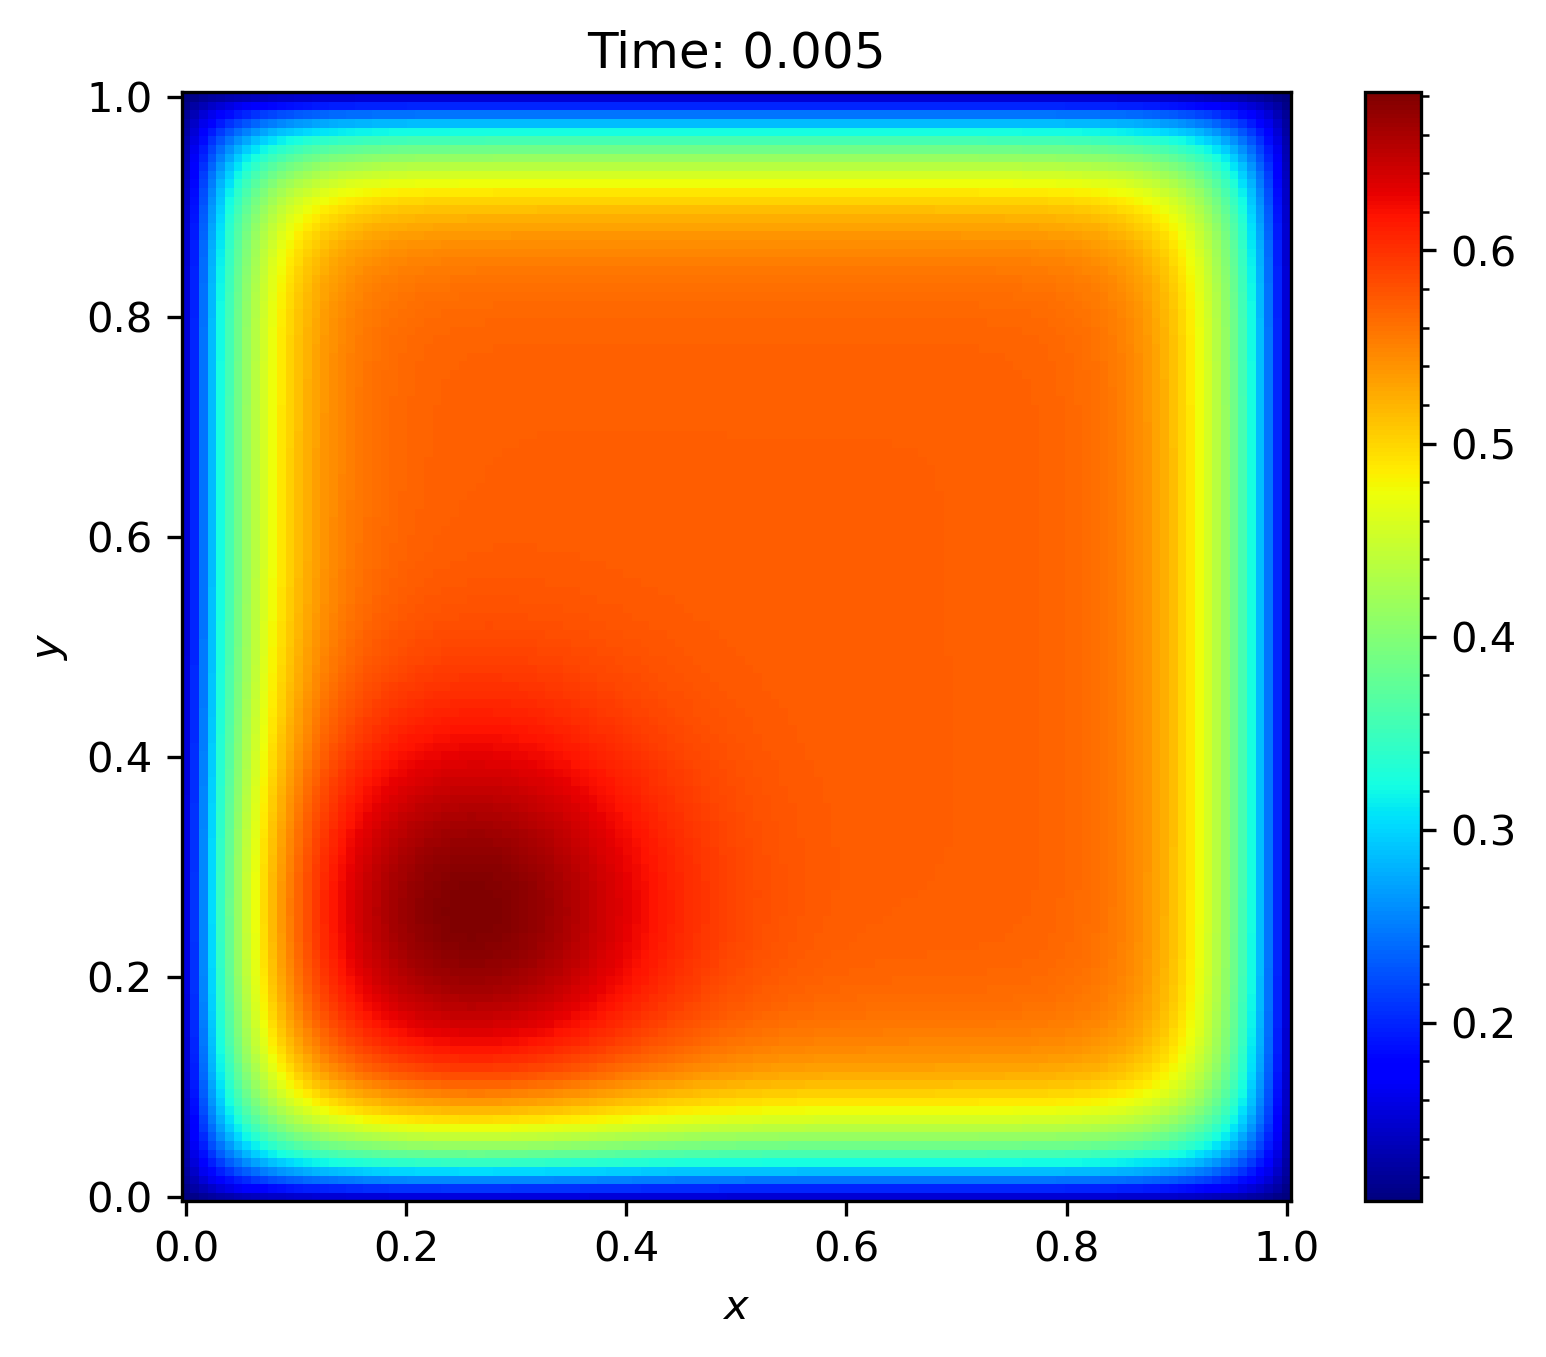
\includegraphics[width=0.5\textwidth]{../code/mini_app/output.png}
  \caption{Output plot}
\end{figure}


NOTICE: this works perfect in my local machine (mac os) but in the cluster there is a problem when running "$MPI\_File\_write\_all$"
which seems to take a lot of time to actually finish running. I assume this has to be 
on how the shared file system of the cluster is handled or latency. Therefore, for running in the cluster I made 
a modified version of the code where I generate a unique binary file for each rank separately, avoiding the shared files problem. Then, the 
resulting files can be combined. I provided the implementation of that in \texttt{code/mini\_app/combination}. Then, for the weak and strong scaling i will use this code. 

\section{Task 6 - Strong Scaling}

For plotting the required statistics, I run the code for each process {1,2,4,8,16} and for each grid size {64,128,512,1024} by making use 
of the provided $strong\_scaling.sh$ batch file and the python util code. 

\begin{figure}[H]
  \centering
  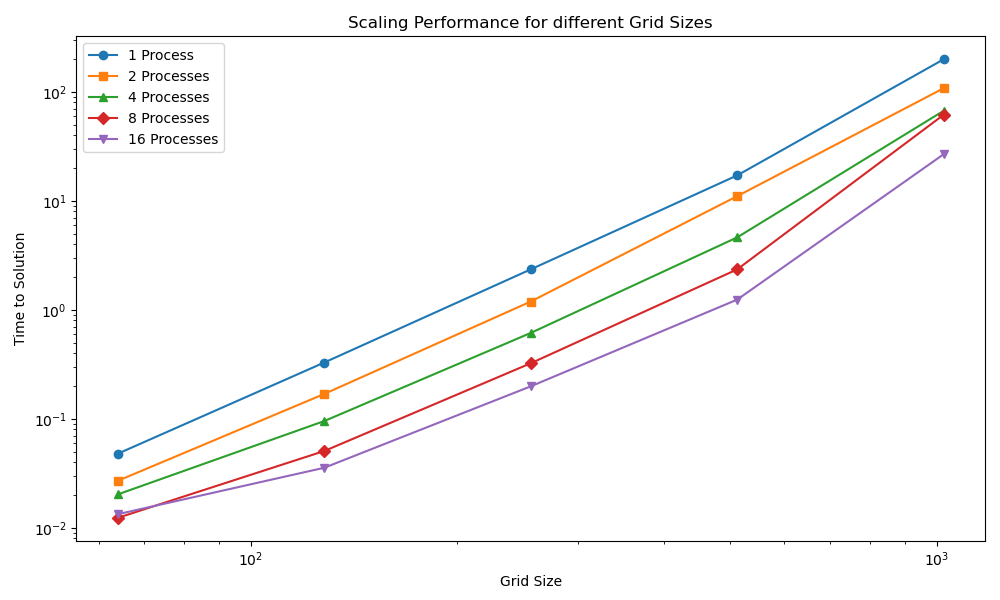
\includegraphics[width=\textwidth]{../code/mini_app/strongscaling/strong_scaling.png}
  \caption{Strong scaling Plot - where the x-axis is the log of the grid size domain and the y-axis the log of the time to solution}
\end{figure}


% Add to preamble:
% \usepackage{placeins}

\FloatBarrier  % Ensures all previous floats are processed
\begin{table}[!h]
\centering
\caption{Scaling Analysis for Resolution 64×64}
\begin{tabular}{cccc}
\hline
Threads & Time (s) & Speedup & Efficiency \\
\hline
1 & 0.05 & 1.00 & 1.00 \\
2 & 0.03 & 1.77 & 0.89 \\
4 & 0.02 & 2.36 & 0.59 \\
8 & 0.01 & 3.88 & 0.48 \\
16 & 0.01 & 3.59 & 0.22 \\
\hline
\end{tabular}
\end{table}
\FloatBarrier

\begin{table}[!h]
\centering
\caption{Scaling Analysis for Resolution 128×128}
\begin{tabular}{cccc}
\hline
Threads & Time (s) & Speedup & Efficiency \\
\hline
1 & 0.33 & 1.00 & 1.00 \\
2 & 0.17 & 1.94 & 0.97 \\
4 & 0.10 & 3.44 & 0.86 \\
8 & 0.05 & 6.48 & 0.81 \\
16 & 0.04 & 9.24 & 0.58 \\
\hline
\end{tabular}
\end{table}
\FloatBarrier

\begin{table}[!h]
\centering
\caption{Scaling Analysis for Resolution 256×256}
\begin{tabular}{cccc}
\hline
Threads & Time (s) & Speedup & Efficiency \\
\hline
1 & 2.35 & 1.00 & 1.00 \\
2 & 1.19 & 1.97 & 0.99 \\
4 & 0.61 & 3.83 & 0.96 \\
8 & 0.32 & 7.26 & 0.91 \\
16 & 0.20 & 11.83 & 0.74 \\
\hline
\end{tabular}
\end{table}
\FloatBarrier

\begin{table}[!h]
\centering
\caption{Scaling Analysis for Resolution 512×512}
\begin{tabular}{cccc}
\hline
Threads & Time (s) & Speedup & Efficiency \\
\hline
1 & 17.11 & 1.00 & 1.00 \\
2 & 11.03 & 1.55 & 0.78 \\
4 & 4.62 & 3.70 & 0.93 \\
8 & 2.35 & 7.28 & 0.91 \\
16 & 1.24 & 13.79 & 0.86 \\
\hline
\end{tabular}
\end{table}
\FloatBarrier

\begin{table}[!h]
\centering
\caption{Scaling Analysis for Resolution 1024×1024}
\begin{tabular}{cccc}
\hline
Threads & Time (s) & Speedup & Efficiency \\
\hline
1 & 198.76 & 1.00 & 1.00 \\
2 & 107.90 & 1.84 & 0.92 \\
4 & 66.96 & 2.97 & 0.74 \\
8 & 61.60 & 3.23 & 0.40 \\
16 & 26.76 & 7.43 & 0.46 \\
\hline
\end{tabular}
\end{table}
\FloatBarrier

Comparing table by table with the results with the project 3, we can see that the overall 
performance is much better for openMPI for a size smaller than 512x512. In that point and on, the performance
of the openMP implementation shows better results. This show us again the trade-offs between shared and distributed memory parallelization approaches. 
For problem sizes smaller than 512x512, OpenMPI demonstrates superior performance due to its efficient process management, independent memory spaces, and better cache utilization, as each process maintains its own cache. 
However, this advantage shifts at larger problem sizes (512x512 and above) where OpenMP shared memory model proves more effective. 
This could be attributed to the changing memory vs computation bottlenecks. In smaller problems, OpenMP's thread creation overhead and cache coherency management represent a significant portion of the execution time, 
while OpenMPI process-based approach better amortizes these overheads. As the problem size grows, OpenMP's shared memory access becomes more efficient than OpenMPI message passing, which incurs 
increased communication overhead due to larger data transfers between processes. 


\section{Task 7 - Weak Scaling}

For this, we need to increment the size of the grid proportionally to the process increment such that the amount of work stays constant: $n^2 = p * (n\_base)^2$ where n is the 
calculated grid size for processes p and $n\_base$ is the base grid size. For example, 
if the base is 64 for 1 process, then we need $\approx$ 90 for two processes to get the same amount of cells per process. 

As we will see in the following graph and table, the results get worst while increasing the base grid size. Showing again the memory bandwidth 
constraint effects in the parallelization. In particular, while for the 64 and 128 sizes the runtime increases $\approx$ 3.7 times the base runtime 
which can be due to overheads of parallelization or Amdahl's law, for the 256 grid size, the increment rises to $\approx$ 11.5 times the base. 

\begin{figure}[H]
  \centering
  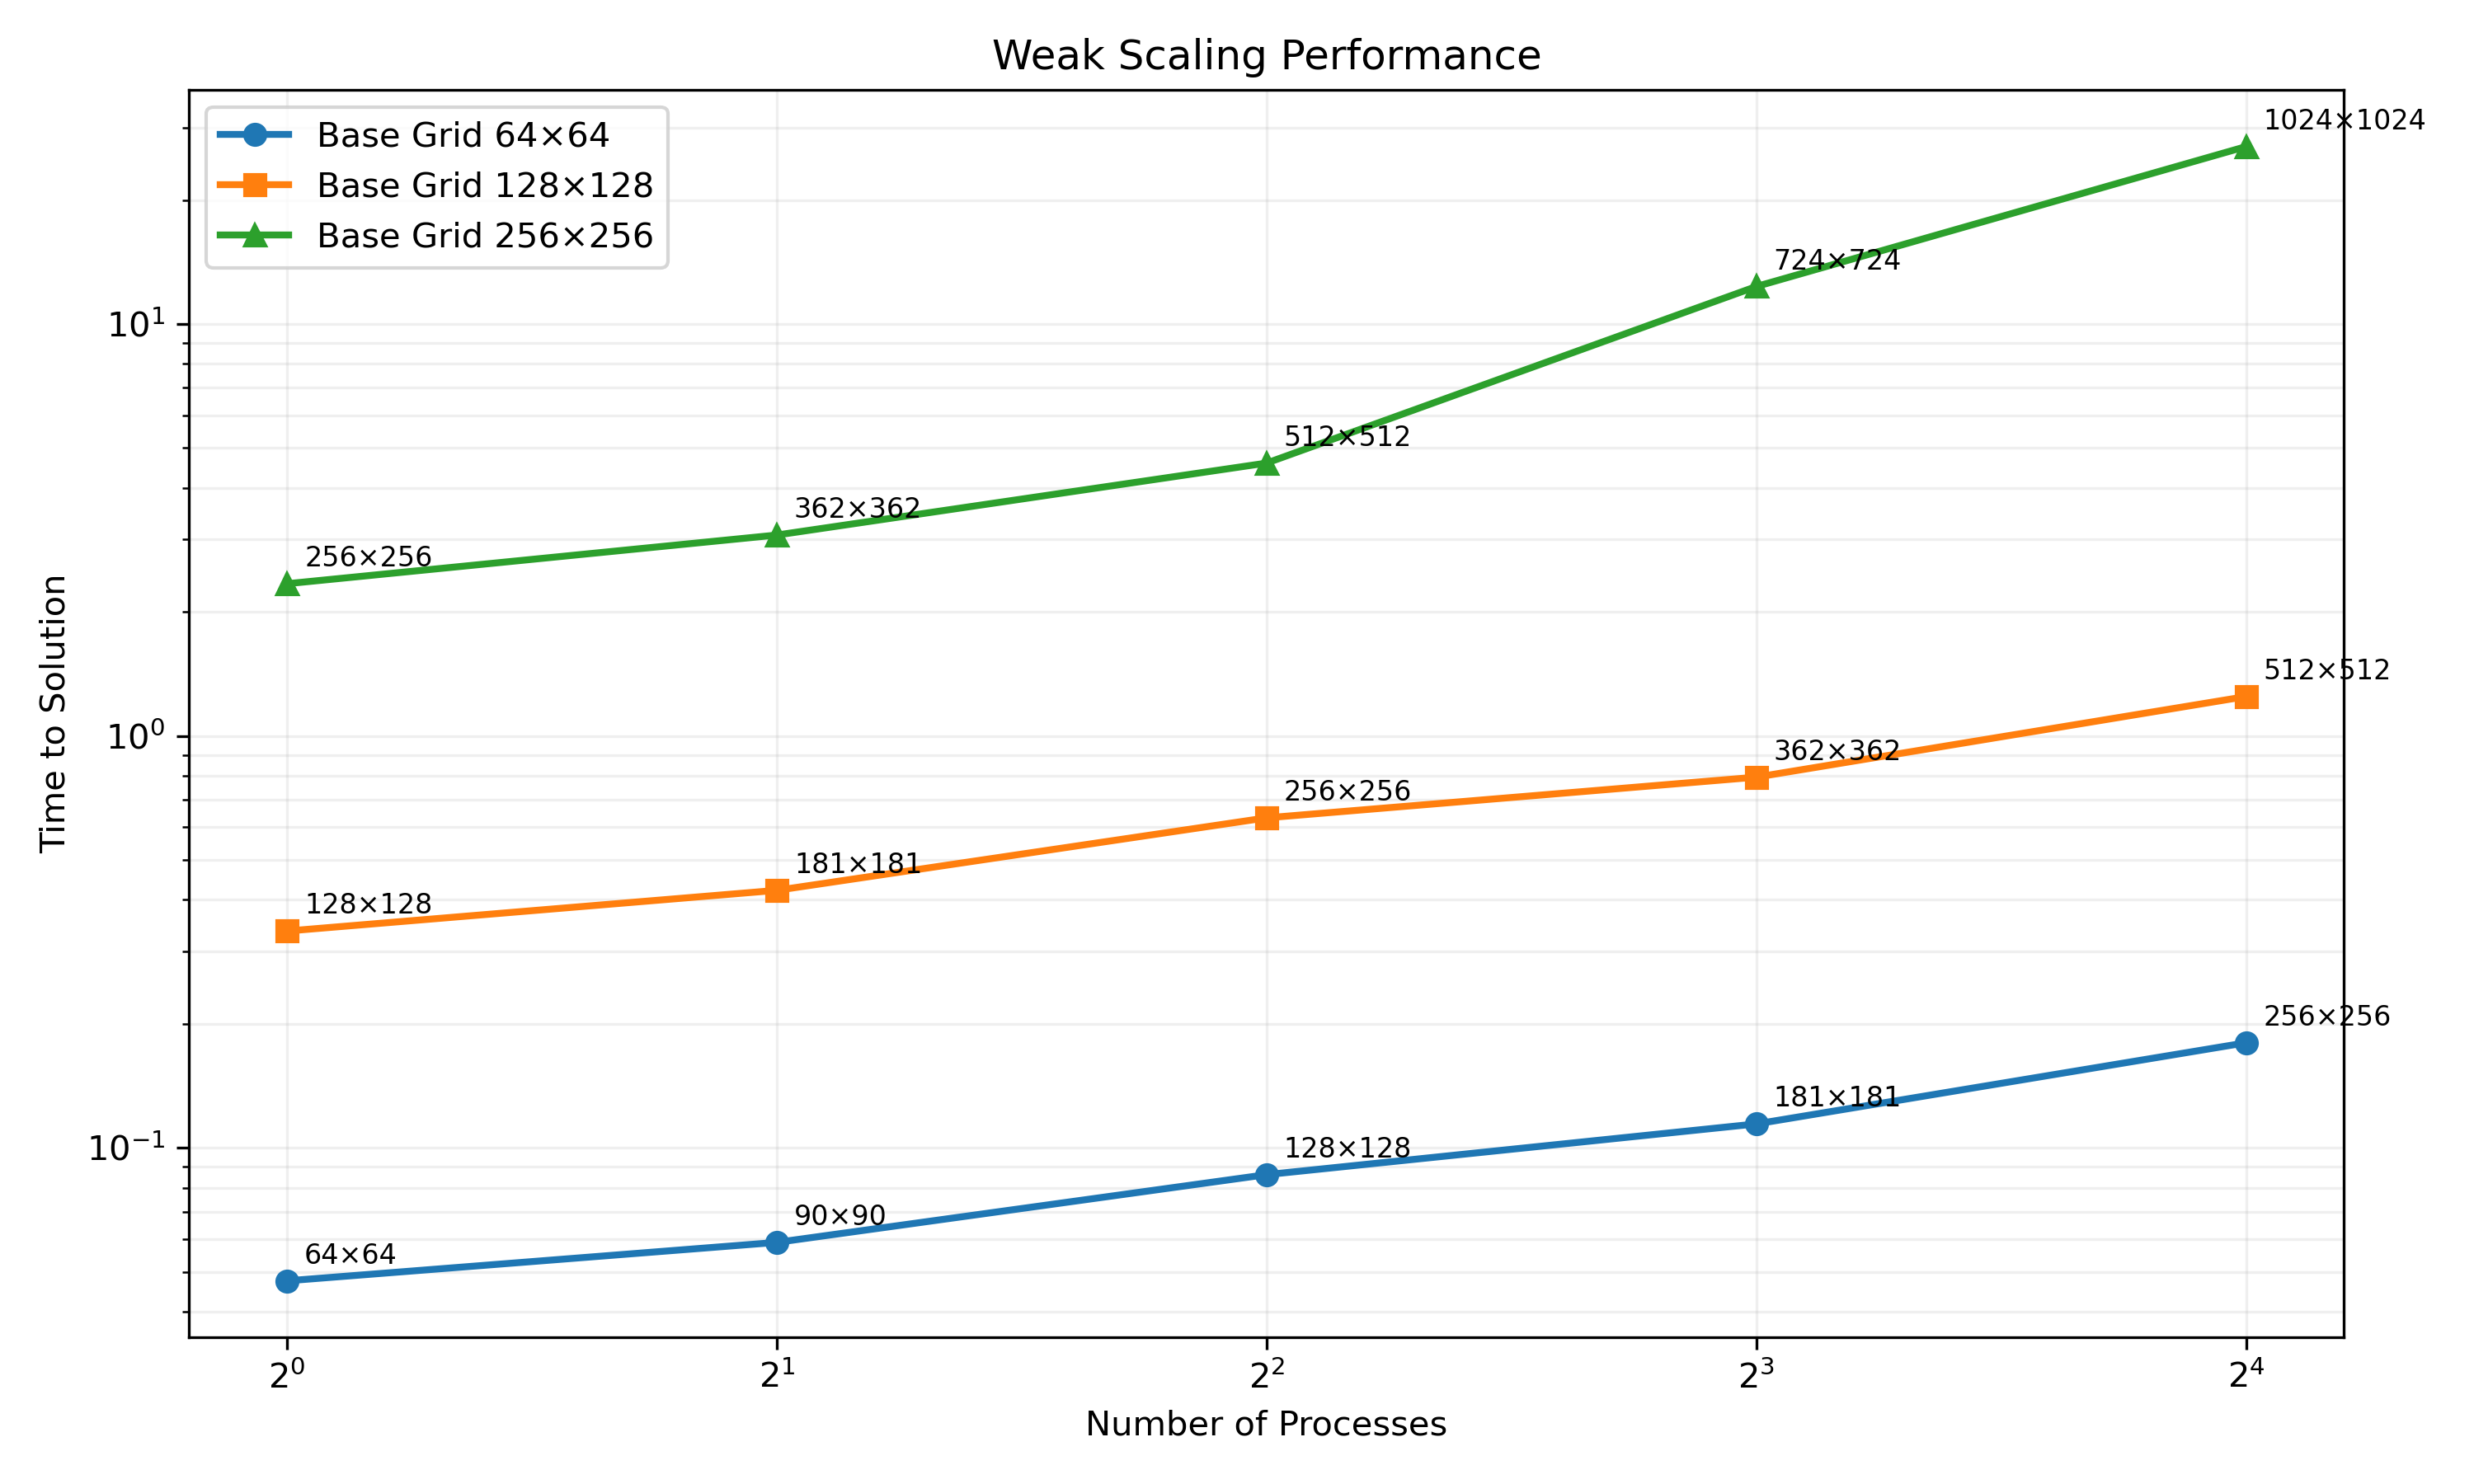
\includegraphics[width=\textwidth]{../code/mini_app/weakscaling/weak_scaling.png}
  \caption{Weak scaling Plot - where the x-axis is the log of the processes and the y-axis the log of the time to solution}
\end{figure}

\begin{table}[!ht]
  \centering
  
  \caption{Weak Scaling Analysis - Base Grid 64×64}
  \begin{tabular}{ccccc}
  \hline
  Processes & Grid Size & CG Iterations & Newton Iterations & Time (s) \\
  \hline
  1 & 64×64 & 1333 & 301 & 0.048 \\
  2 & 90×90 & 1694 & 300 & 0.059 \\
  4 & 128×128 & 2225 & 300 & 0.086 \\
  8 & 181×181 & 3006 & 300 & 0.114 \\
  16 & 256×256 & 4109 & 300 & 0.180 \\
  \hline
  \end{tabular}
  
  \vspace{1em}
  
  \caption{Weak Scaling Analysis - Base Grid 128×128}
  \begin{tabular}{ccccc}
  \hline
  Processes & Grid Size & CG Iterations & Newton Iterations & Time (s) \\
  \hline
  1 & 128×128 & 2232 & 300 & 0.336 \\
  2 & 181×181 & 3010 & 300 & 0.422 \\
  4 & 256×256 & 4107 & 300 & 0.633 \\
  8 & 362×362 & 5654 & 300 & 0.794 \\
  16 & 512×512 & 7817 & 301 & 1.246 \\
  \hline
  \end{tabular}
  
  \vspace{1em}
  
  \caption{Weak Scaling Analysis - Base Grid 256×256}
  \begin{tabular}{ccccc}
  \hline
  Processes & Grid Size & CG Iterations & Newton Iterations & Time (s) \\
  \hline
  1 & 256×256 & 4100 & 300 & 2.342 \\
  2 & 362×362 & 5663 & 300 & 3.075 \\
  4 & 512×512 & 7806 & 300 & 4.597 \\
  8 & 724×724 & 10882 & 304 & 12.336 \\
  16 & 1024×1024 & 16065 & 338 & 26.968 \\
  \hline
  \end{tabular}
  
  \end{table}


\section{Exercise 2: Python for High-Performance Computing}
\subsection{Sum of ranks: MPI collectives}
MPI for python supports pickle-based communication of generic python objects or direct array data (as numpy arrays) as buffer-provided objects:
\begin{itemize}
  \item For the pickle - based communication we use all-lowercase methods name, and we can send an object with different types to be serialized, converted into byte stream
  send these bytes between processes, unpickle back into objects and perform the respective operation: 

  For implementing this example with the sum of ranks and following the provided example, I first set up the MPI world communication and then get the rank and size of the process. 
  For this method, we do not need to do anything else with the ranks since it will be managed by python (at the cost of higher runtime), therefore, I pass the ranks to the $allreduce$ function with 
  the specified sum operation. Then, it will print out the sum of ranks and the time taken to perform the operation. The truth time is the $\frac{p*(p-1)}{2}$ since we have p ranks. For example, with 8 processes we
  get 28, in 0.0341 sec (on the cluster).

  \item For the buffer-like objects we use directly the upper-case and MPI directly accesses the memory where the NumPy array is stored, transfers the raw memory between processes, 
  performs the operations directly in the buffers with no need of conversions or serialization. Now, for this implementation the same ranks are converted to a rank array and I define a 
  sum of ranks array to store the solution. Then, the $Allreduce$ function is called with the rank array, the sum of ranks array, the specified sum operation.
  Finally, it will print out the sum of ranks and the time taken to perform the operation. Continuing with the 8 processes example, we get again 28, but in 0.000154 sec (on the cluster).
\end{itemize}
\subsection{Ghost cell exchange between neighboring processes}
To implement this I firstly write down the procedure of a little example with 4 processes. Then, I implemented the code following the procedure. Therefore, i will proceeed to comment the code
with this example on mind:

I first initialize the communicator and get the rank and the number of processes as always. Then, we need to calculate the grid dimensions to be evenly distributed. This can be achieved 
by using $MPI.Compute_dims(size, [0,0])$ where size is the number of processes and the arrays by passing [0,0] allows mpi to determine by itself
the even distribution of processes which in the example of 4 processes this is 2x2. 
Then, by setting period True and reorder to False (default row major) we create the Cartesian communicator.
This will create a mapping from [1,2,3,4] processes to:
$\begin{bmatrix}
[1] & [2] \\
[3] & [4]
\end{bmatrix}$ 

and then, $\begin{bmatrix}
          [0,0] & [0,1] \\
          [1,0] & [1,1]
          \end{bmatrix}$  since $Get\_coords$ will give us the coordinates of the process which in the example of 4 processes, the process 1 will be mapped to [0,0], process 2 to [0,1], process 3 to [1,0] and process 4 to [1,1] - row major ordering.

Having this in mind, i step up a neighbours dictionary to store the north, south, east and west neighbours of each process, in which each corresponding key is the rank of such a neighbour. For example, for 
rank 0, we obtain its coordinates with $cart\_comm.Get\_coords(rank)$ which is [0,0]. Then, we get the neighbour in the north direction with $cart\_comm.Get\_cart\_rank((coords[0]-1, coords[1]))$ which is process 2 \footnote{
  the reason why coords[0]-1 can be seen clearly in the previous matrix, since the upper value in a periodic case for the border will be the bottom one in the same column
}. For the south neighbour we get $cart\_comm.Get\_cart\_rank((coords[0]+1, coords[1]))$ which is process 2. For the east neighbour we get $cart\_comm.Get\_cart\_rank((coords[0], coords[1]+1))$ which is process 1.
For the west neighbor we get $cart\_comm.Get\_cart\_rank((coords[0], coords[1]-1))$ which is process 1 for the same argument as process 2 is north one.
Then, I create a buffer to store the ranks that we receive from the neighbors.

\begin{verbatim}
  neighbors = {
    'north': cart_comm.Get_cart_rank((coords[0]-1, coords[1])), 
    'south': cart_comm.Get_cart_rank((coords[0]+1, coords[1])),
    'east': cart_comm.Get_cart_rank((coords[0], coords[1]+1)),
    'west': cart_comm.Get_cart_rank((coords[0], coords[1]-1))
}
\end{verbatim}

Once this is done, then we already have the "ids" of each neighbor of each process. I print them and continue with the receiving and sending part of the implementation. 
As a good practice I start with the receiving to avoid deadlocks, however I use the non-blocking method for each send and receive anyway. Also, using buffer-provider objects.
To do set up the receiving I create for each neighbor dictionary key a buffer to store the ranks that we receive from the neighbors. Then, I create a request list to store the requests for each send and receive.
For the receive then the source is the neighbor rank for each neighbor and the storage is the mentioned buffer. 
The idea for sending is symmetric, the message is the rank array and the destination is each neighbor. The file can be seen in the $hpc\_python/ghost.py$ file.

This is the following result for the example with 4 processes as commented in the example:

\begin{verbatim}
  process 2 coords=[1, 0] 
  neighbors={'north': 0, 'south': 0, 'east': 3, 'west': 3}
  Received: north=0, south=0, east=3, west=3
  
  process 3 coords=[1, 1]
  neighbors={'north': 1, 'south': 1, 'east': 2, 'west': 2}
  Received: north=1, south=1, east=2, west=2
  
  process 0 coords=[0, 0]
  neighbors={'north': 2, 'south': 2, 'east': 1, 'west': 1}
  Received: north=2, south=2, east=1, west=1
  
  process 1 coords=[0, 1]
  neighbors={'north': 3, 'south': 3, 'east': 0, 'west': 0}
  Received: north=3, south=3, east=0, west=0
  \end{verbatim}

\subsection{A self-scheduling example: Parallel Mandelbrot}
For this implementation I will explain each function. We are given the tasks 
already thanks to $get\_tasks$ function, which divides the domain into $ntasks$
patches and for each of them it creates a $mandelbrot\_patch$ object that contains the necessary information
for $do\_task$ method to run the task. Therefore, we need to use the manager to assigned them, wait for the result, 
keep assigning them until finished everything, combined them and print them. 

Therefore, the manager first needs the process number to see how many workers have, 
the status will provide to be very useful in both cases to know the source and the message tag, 
I also create a list of the completed tasks to store them, I copy the tasks queue, keep a count of them and the worker status list where
I consider False as idle and True as busy. For each worker, I do the initial assignment of the tasks by sending a message with the task, the 
worker id as destination, and the tag as given. Then I set that worker state as busy and add the tasks in progress count to 1. 

So now we know that as this counts keeps being over 0 then there are work running. However, now we need to check for the work to finish. 
For this, I set up a receive method for any source with the task done tag, when we receive this message then we know that the worker is done 
his tasks, and it is returning it to us. \footnote{\url{https://stackoverflow.com/questions/4348900/mpi-recv-from-an-unknown-source}}
Since we do not know his ID, we can use the status to get it and I add a count up for its id to return the final statistics. I reduce the count of progress tasks 
and set the worker to idle again. I store the completed tasks to be combined and return at the end. However, we first need to keep sending tasks if we have 
more in the queue. When all of them are complete. Then the manager can finally return the list of completed tasks. 

For the workers, we can simply first get the status and wait for manager orders for any tag since we start with an initial task but later 
on we need to wait for getting the done message. Therefore, after that, we can use the $status.Get\_tag()$ to check if we should break or keep going 
according to the tag. If the manager does not notify that we are done, then we do the work over the given task and send it back to manager when it is finished. 

\begin{figure}[H]
  \centering
  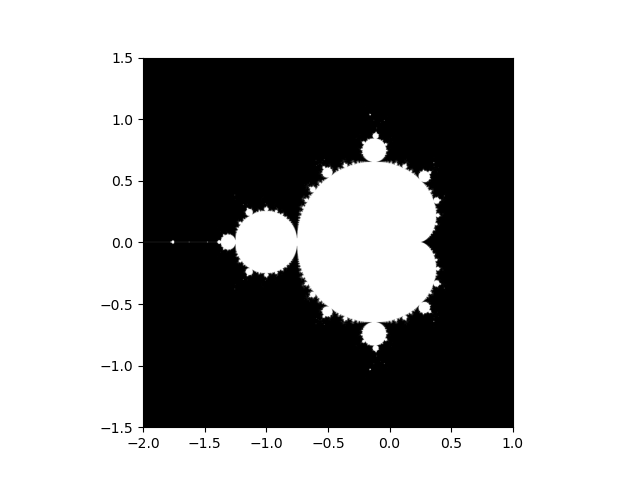
\includegraphics[width=\textwidth]{../code/hpc_python/mandelbrot.png}
  \caption{Mandelbrot Plot}
\end{figure}

Now, for the scaling studies as required: 


\begin{figure}[H]
  \centering
  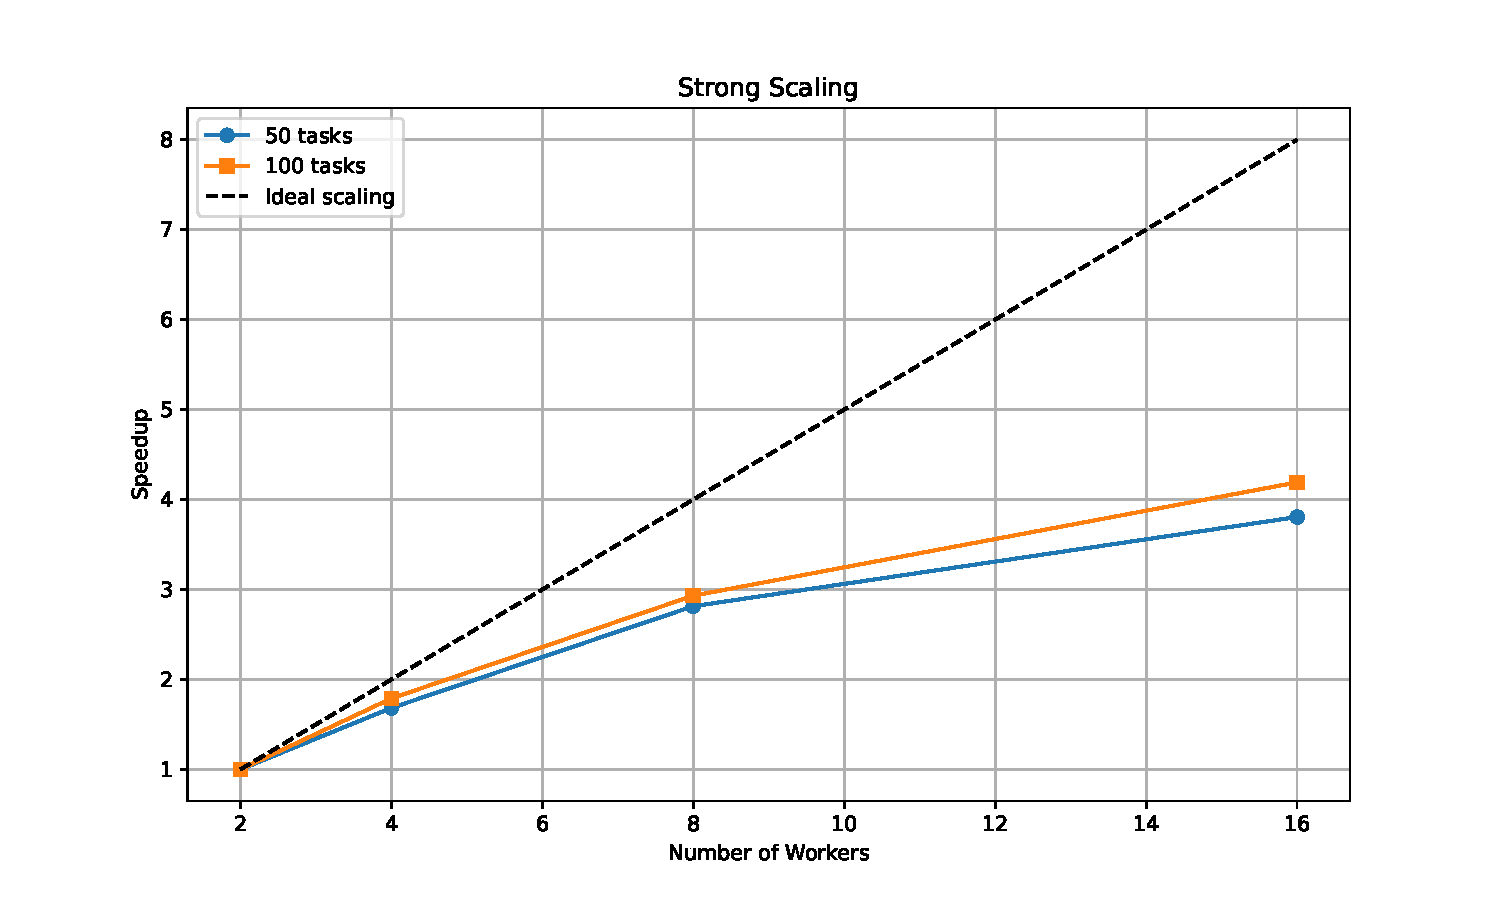
\includegraphics[width=\textwidth]{../code/hpc_python/scaling_study.pdf}
  \caption{Strong Scaling: Speedup vs Number of Workers}
\end{figure}

\begin{table}[!ht]
  \centering
  \caption{Strong Scaling Results}
  \begin{tabular}{cccc}
  \hline
  Workers & Tasks & Runtime (s) & Speedup \\
  \hline
  2 & 50 & 13.47 & 1.00 \\
  4 & 50 & 8.00 & 1.68 \\
  8 & 50 & 4.79 & 2.81 \\
  16 & 50 & 3.54 & 3.80 \\
  \hline
  2 & 100 & 13.44 & 1.00 \\
  4 & 100 & 7.51 & 1.79 \\
  8 & 100 & 4.58 & 2.93 \\
  16 & 100 & 3.21 & 4.19 \\
  \hline
  \end{tabular}
  \end{table}

As we can see, the efficiency of the implementation increases with the size of the task but far from perfect. 
The overhead costs increases with the number of workers and the manager can end up being a problem more than a virtue if we can directly assign 
tasks to each process. 




\end{document}
